\documentclass[12pt]{article}

% Packages 
\usepackage{amsmath}
\usepackage{datetime}
\usepackage{graphicx}
\usepackage{listings}
\usepackage{gensymb}

\graphicspath{{./images/}}

\newdate{date}{28}{03}{2022}
\title{
    Assignment 25-26 

    \large{
        ME EN 6240 Advanced Mechatronics
    }  
}
    
\author{
        Ryan Dalby
}
\date{\displaydate{date}}


\begin{document}
\maketitle

\section*{Chapter 25, Exercise 2}
\begin{itemize}
    \item[a.] 
    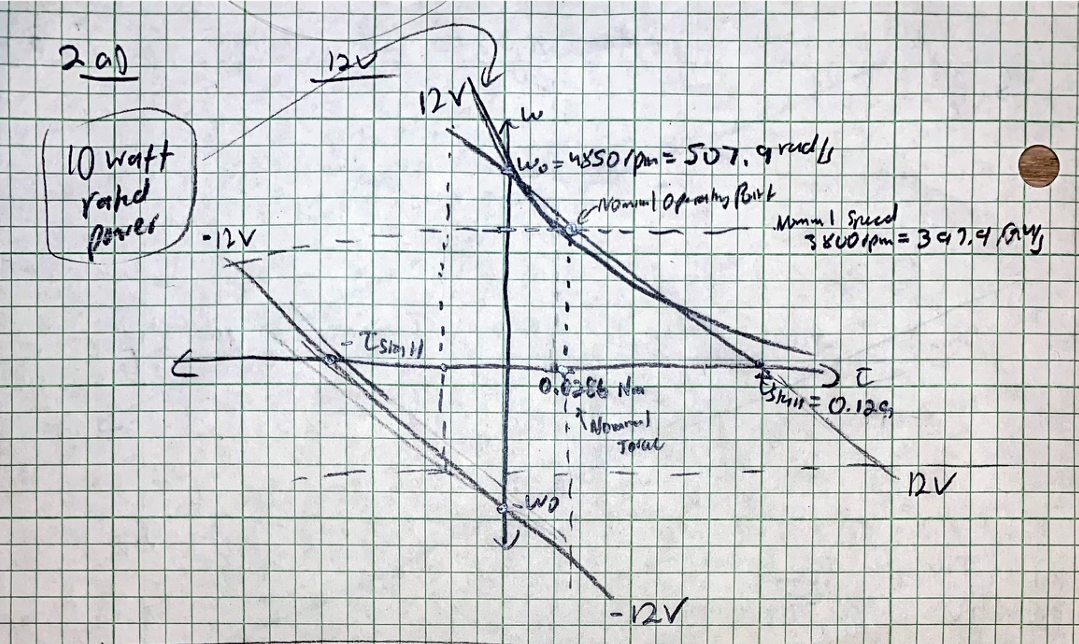
\includegraphics[width=4.8in]{25_2a.png}

    \item[b.] 
    The torque constant differs for each motor because the different versions have different windings and thus the relation between torque and current differs based on the chosen model.

    \item[c.] 
    $\eta_{max} = (1 - \sqrt{\frac{I_0}{I_{stall}}})^2 = 0.8664$

    Value listed:  $\eta_{max} = 0.87$

    \item[d.] 
    $T_e = \frac{L}{R} = 0.0001092 s = 0.1092 ms$

    $\frac{T_e}{T_m} = \frac{0.1092ms}{4.25ms} = 0.026$

    \item[e.] 
    $B = \frac{k_t^2}{R} = 0.000253 Nms$

    \item[f.] 
    $k_m = \frac{k_t}{\sqrt{R}} = 0.0159 Nm/\sqrt{W}$

    \item[g.] 
    11 commutator segments for these motors

    \item[h.] 
    118742, 118743, 118746 are considered stock program so are likely to be in stock

\end{itemize}

\section*{Chapter 25, Exercise 3}
N independent entries:
\begin{itemize}
    \item 
    $V_{nom}$

    \item 
    $R$

    \item 
    $L$

    \item 
    $J$

    \item 
    $k_t$

    \item 
    $P$

    \item 
    $I_0$ (or not included since we are not considering friction ($I_0 = 0$))

\end{itemize}

20-N dependent entries:
\begin{itemize}
    \item 
    $I_{stall} = V_{nom}/R$

    \item
    $k_e = k_t$

    \item
    $k_s = \frac{1}{k_e}$

    \item
    $k_m = \frac{k_t}{\sqrt{R}}$

    \item
    $B = \frac{k_t^2}{R}$

    \item 
    $\tau_{stall} = k_t I_{stall}$

    \item 
    $I_{cont} = P/V_{nom}$

    \item 
    $\tau_{cont} = k_t I_{cont}$

    \item 
    $\omega_0 = \frac{V_{nom}}{k_t}$

    \item 
    $T_m = \frac{J R}{k_t^2}$

    \item 
    $T_e = \frac{L}{R}$

    \item 
    $P_{max} = \frac{1}{4} \tau_{stall} \omega_0$
    
    \item 
    $\eta_{max} = (1 - \sqrt{\frac{I_0}{I_{stall}}})^2$

\end{itemize}

\section*{Chapter 25, Exercise 7}
Requirements: 
\begin{itemize}
    \item 
    $\tau_{stall} > 0.1 Nm$

    \item 
    $\omega\rvert_{0.01 Nm} = 5 rps = 300 rpm$

    \item
    Continuous operation while producing 0.02 Nm
\end{itemize}
And then choose lowest power motor that meets requirements.

\vspace{0.1in}
{\setlength{\parindent}{0cm}
Initially checked $\tau_{stall}$ for each of the motors and found that the 3 Watt motor has $\tau_{stall} = 0.0105 Nm \not> 0.1 Nm$ thus it cannot be considered. 

The 10W, 20W, and 90W motor all meet the stall specification with 0.131 Nm, 0.225 Nm, and 0.929 Nm respectively.
These 3 motors also meet the continuos operation specification by having at least 0.02Nm as the max continuos torque with 0.0282 Nm, 0.0205 Nm, 0.0731 Nm respectively.

Using $\omega = \omega_0 - \frac{\omega_0}{\tau_{stall}}\tau$ it can be found that the 10W motor can produce up to $4600 rpm = 4980 rpm - \frac{4980 rpm}{0.131 Nm}(0.01 Nm)$ at 0.01 Nm which exceeds the 300rpm specification.

Thus the 10 W motor is the selected motor.
}
\section*{Chapter 25, Exercise 8}
\begin{center}
    
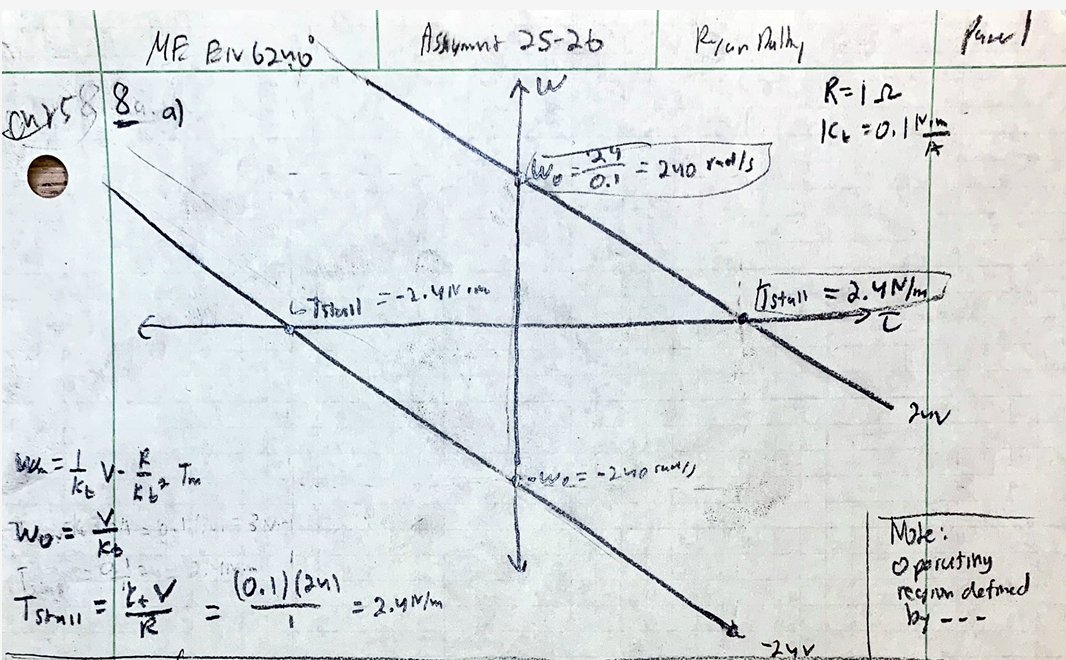
\includegraphics[width=5.2in]{25_8a.png}

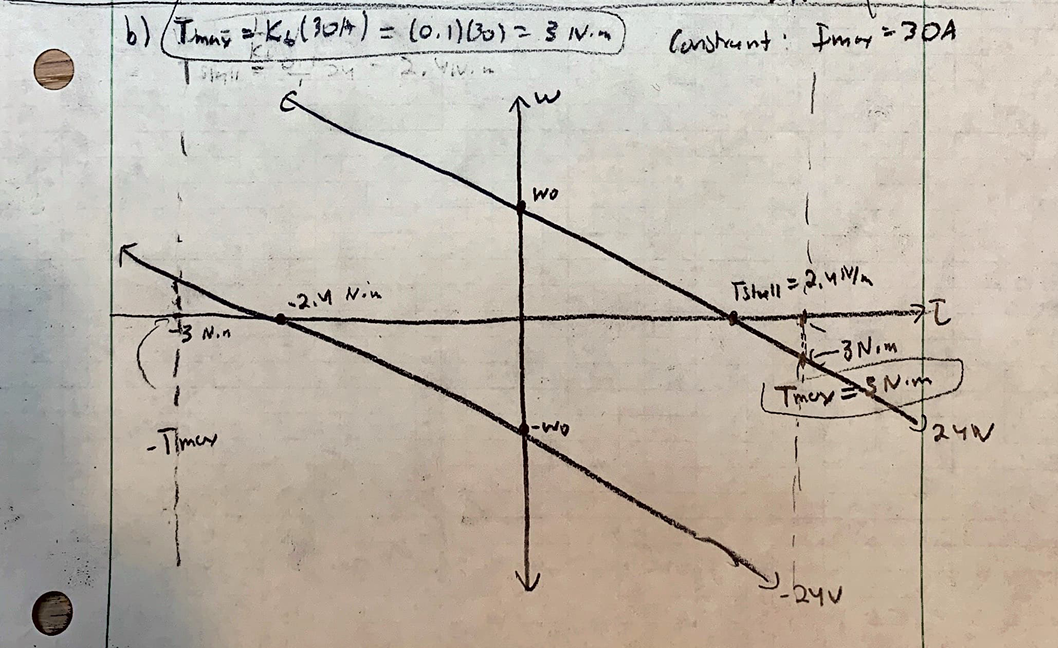
\includegraphics[width=5.2in]{25_8b.png}

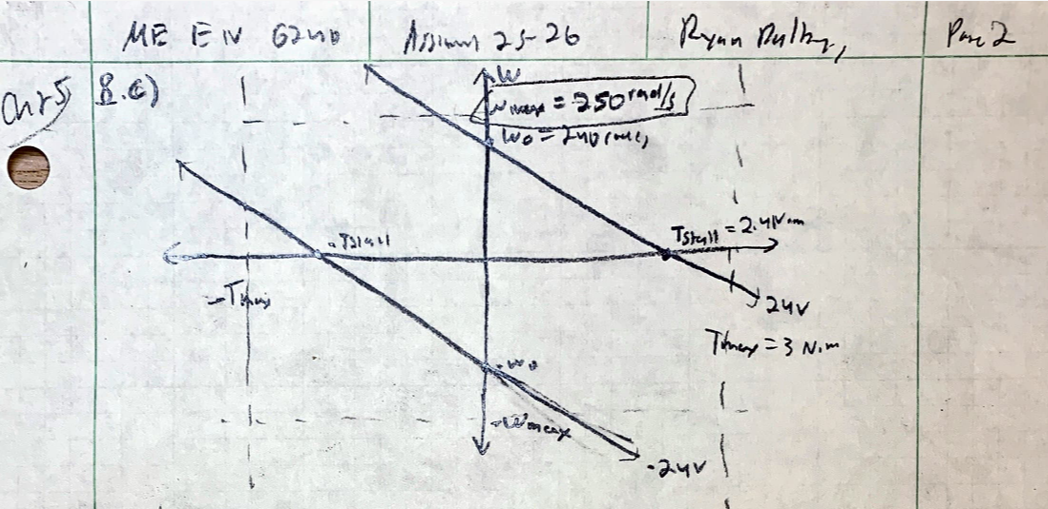
\includegraphics[width=5.2in]{25_8c.png}

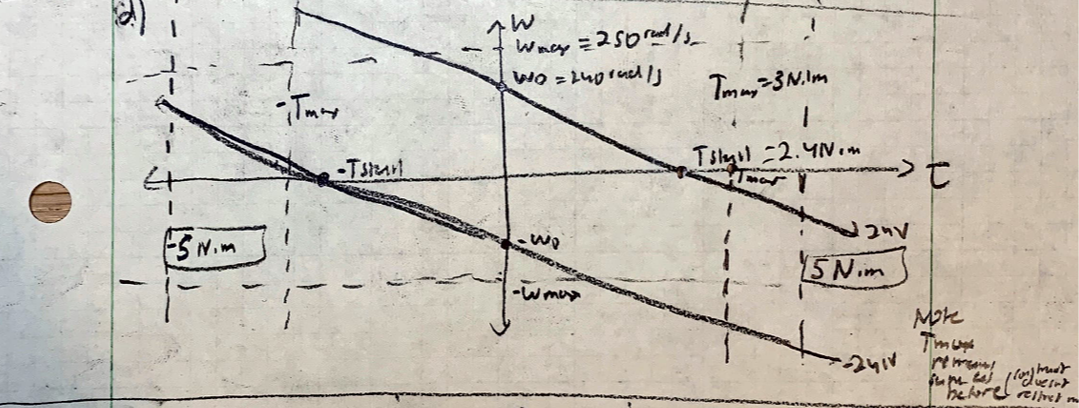
\includegraphics[width=5.2in]{25_8d.png}

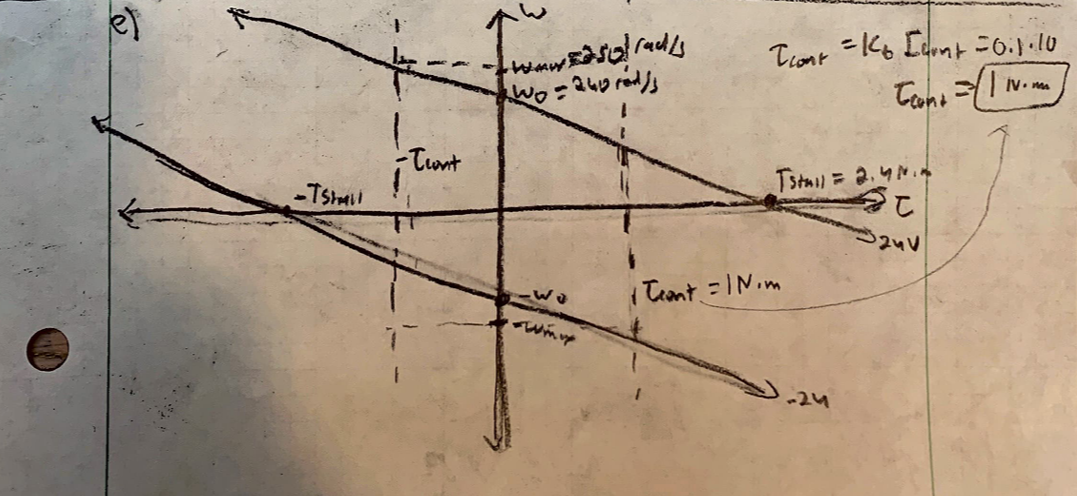
\includegraphics[width=5.2in]{25_8e.png}

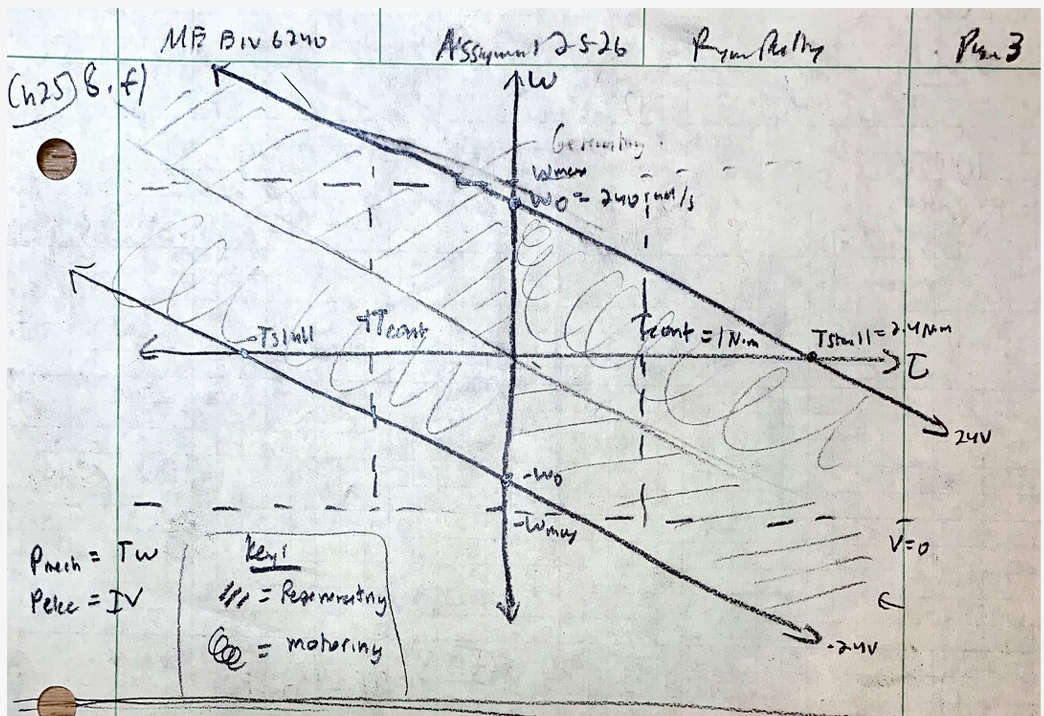
\includegraphics[width=5.2in]{25_8f.png}

\end{center}

\section*{Chapter 26, Exercise 1}
1-stage:
\begin{itemize}
    \item 
    10:15 gear train has $G=1.5$ and $\eta = 0.85$

    \item 
    10:20 gear train has $G=2$ and $\eta = 0.8$

    \item 
    15:20 gear train has $G=1.33$ and $\eta = 0.9$
\end{itemize}

\noindent
2-stage (Note that repeated combinations were excluded as there is rarely any use for these as essentially efficiency loss occurs with no change in gearing):
\begin{itemize}
    \item 
    10:15:20 gear train has $G=2$ and $\eta = 0.765$

    \item 
    10:20:15 gear train has $G=1.5$ and $\eta = 0.72$

    \item 
    15:10:20 gear train has $G=1.33$ and $\eta = 0.68$
\end{itemize}

\section*{Chapter 26, Exercise 4}
\begin{itemize}
    \item[a.] 
    Given the specifications, we can create a model for the system dynamics.
    (Note that $F_{both}$ is the force of the ground pushing back on both of the wheels, $F_{single}$ the force of the ground pushing back on a single wheel, $r$ is the radius of the wheel, $\tau$ is the torque at the wheel of a single wheel, $F_b$ is the viscous damping force, $v$ is the translational velocity of the robot, $m$ is the total mass of the robot and $g$ is the gravitational constant.)

    Also note that $F_{single} = F_{both}/2$, $\tau = F_{single} r$, $v = \omega r$
    Using a force balance in the x direction (which is taken to be parallel with the slope the robot drives up from a side view) gives:
    \[
        \sum F_x = mg\sin(20\degree) - F_{both} + F_B = 0
    \]
    With $F_B = (10 Ns/m) v$ 
    \[
        F_{both} = mg\sin(20\degree) + 10v
    \]
    \[
        F_{single} = \frac{mg\sin(20\degree) + 10v}{2}
    \]
    \[
        \tau = \frac{mgr\sin(20\degree) + 10vr}{2}
    \]
    With $v = 0.2 m/s$, $m=2kg$, $r=0.04m$, $g=9.81m/s^2$
    \[
        \tau = 0.174 Nm
    \]

    $\omega_{in}$ is the angular velocity of the motor while $\omega_{out}$ is the angular velocity after the gear train.
    Similarly, $\tau_{in}$ is the torque of the motor while $\tau_{out}$ is the torque after the gear train.

    \textbf{Rephrased requirement:} We want the chosen motor gear head combination to be able to \textbf{continuously} provide (at least) $\tau_{out} = \tau = 0.174 Nm$ while still providing (at least) $\omega_{out} = \frac{v}{r} = \frac{0.2}{0.04} = 5 rad/s = 47.75 rpm$.

    Using $\omega_{out} = \frac{1}{G}\omega_{in}$ and $\tau_{out} = \eta G \tau_{in}$ where $G$ is the gear ratio we can deduce which motor gear train combinations to use.

    First, considering $G = 1$ none of the motors can directly meet the requirement since their max continous torques are not greater than 0.174 Nm.

    For the rest of the gear trains we have $\eta = 0.75$ thus $\omega_{out} = \frac{1}{G}\omega_{in}$ and $\tau_{out} = (0.75) G \tau_{in}$ 

    The following motor gear train combinations can meet the specifications (the gear train output torque speed curve using the original motor specifications is found using $\omega_{out} = \frac{\omega_0}{G} - \frac{\omega_0}{(0.75)G^2\tau_{stall}}\tau_{out}$): 
    \begin{itemize}
        \item 
        3 W Motor ($\tau_{max, continous} = 0.00231 Nm$ (will be used as $\tau_{in}$))
        \begin{itemize}
            \item
            None. (Even with $G=100$, $tau_{out} = 0.173 Nm$ which is less than the requirement)
        \end{itemize}

        \item 
        10 W Motor ($\tau_{max, continous} = 0.0282 Nm$ (will be used as $\tau_{in}$))
        Speed torque curve is: $\omega_{out} = \frac{4980rpm}{G} - \frac{4980rpm}{(0.75)G^2(0.131Nm)}\tau_{out}$
        \begin{itemize}
            \item
            $G=10$, 

            $\tau_{out} = (0.0282) (.75) (10) = 0.212 Nm > 0.174 Nm$

            $\omega_{out} = \frac{4980rpm}{10} - \frac{4980rpm}{(0.75)(10)^2(0.131Nm)}(.174Nm) = 409.80 rpm > 47.75rpm$

            \item
            $G=20$,

            $\tau_{out} = (0.0282) (.75) (20) = 0.423 Nm > 0.174 Nm$

            $\omega_{out} = \frac{4980rpm}{20} - \frac{4980rpm}{(0.75)(20)^2(0.131Nm)}(.174Nm) = 226.95 rpm > 47.75rpm$

            \item
            $G=50$

            $\tau_{out} = (0.0282) (.75) (50) = 1.058 Nm > 0.174 Nm$

            $\omega_{out} = \frac{4980rpm}{50} - \frac{4980rpm}{(0.75)(50)^2(0.131Nm)}(.174Nm) = 96.07 rpm > 47.75rpm$

            \item
            $G=100$

            $\tau_{out} = (0.0282) (.75) (100) = 2.115 Nm > 0.174 Nm$

            $\omega_{out} = \frac{4980rpm}{100} - \frac{4980rpm}{(0.75)(100)^2(0.131Nm)}(.174Nm) = 48.92 rpm > 47.75rpm$

        \end{itemize}

        \item 
        20 W Motor ($\tau_{max, continous} = 0.0205 Nm$ (will be used as $\tau_{in}$))
        Speed torque curve is: $\omega_{out} = \frac{9660rpm}{G} - \frac{9660rpm}{(0.75)G^2(0.225Nm)}\tau_{out}$
        \begin{itemize}
            \item
            $G=20$

            $\tau_{out} = (0.0205) (.75) (20) = 0.212 Nm > 0.174 Nm$

            $\omega_{out} = \frac{9660rpm}{20} - \frac{9660rpm}{(0.75)(20)^2(0.225Nm)}(0.174Nm) = 458.10 rpm > 47.75 rpm$

            \item
            $G=50$

            $\tau_{out} = (0.0205) (.75) (50) = 0.769 Nm > 0.174 Nm$

            $\omega_{out} = \frac{9660rpm}{50} - \frac{9660rpm}{(0.75)(50)^2(0.225Nm)}(0.174Nm) = 189.22 rpm > 47.75 rpm$

            \item
            $G=100$

            $\tau_{out} = (0.0205) (.75) (100) = 1.538 Nm > 0.174 Nm$

            $\omega_{out} = \frac{9660rpm}{100} - \frac{9660rpm}{(0.75)(100)^2(0.225Nm)}(0.174Nm) = 95.60 rpm > 47.75 rpm$

        \end{itemize}

        \item 
        90 W Motor ($\tau_{max, continous} = 0.0731 Nm$ (will be used as $\tau_{in}$))
        Speed torque curve is: $\omega_{out} = \frac{7180rpm}{G} - \frac{7180rpm}{(0.75)G^2(0.929Nm)}\tau_{out}$
        \begin{itemize}
            \item
            $G=10$

            $\tau_{out} = (0.0731) (.75) (10) = 0.548 Nm > 0.174 Nm$

            $\omega_{out} = \frac{7180rpm}{10} - \frac{7180rpm}{(0.75)(10)^2(0.929Nm)}(0.174Nm) = 700.07 rpm > 47.75 rpm$

            \item
            $G=20$

            $\tau_{out} = (0.0731) (.75) (20) = 1.097 Nm > 0.174 Nm$

            $\omega_{out} = \frac{7180rpm}{20} - \frac{7180rpm}{(0.75)(20)^2(0.929Nm)}(0.174Nm) = 354.52 rpm > 47.75 rpm$

            \item
            $G=50$

            $\tau_{out} = (0.0731) (.75) (50) = 2.741 Nm > 0.174 Nm$

            $\omega_{out} = \frac{7180rpm}{50} - \frac{7180rpm}{(0.75)(50)^2(0.929Nm)}(0.174Nm) = 142.88 rpm > 47.75 rpm$

            \item
            $G=100$

            $\tau_{out} = (0.0731) (.75) (100) = 5.482 Nm > 0.174 Nm$

            $\omega_{out} = \frac{7180rpm}{100} - \frac{7180rpm}{(0.75)(100)^2(0.929Nm)}(0.174Nm) = 71.62 rpm > 47.75 rpm$

        \end{itemize}
    \end{itemize}

    \item[b.] 
    I would choose the 10W motor with the $G = 10$ gear train to optimize the cost since this is the lowest power rating motor and smallest gear train that meets the requirements.

    \item[c.] 
    Noting that $\eta = \frac{\tau_{out} \omega_{out}}{P} = \frac{(0.174Nm) \omega_{out}}{P}$ we just look at the largest $\omega_{out}$ gear train for the 10W, 20W, and 90W motors.

    \begin{itemize}
        \item 
        $P = 10 W$ Motor with $G = 10$:

        $409.80 rpm = 42.91 rad/s$

        $\eta = 0.747$

        \item 
        $P = 20 W$ Motor with $G = 20$:

        $458.10 rpm = 47.97 rad/s$

        $\eta = 0.417$

        \item 
        $P = 90 W$ Motor with $G = 10$:

        $700.07 rpm = 73.38 rad/s$

        $\eta = 0.142$
        
    \end{itemize}

    I would choose the 10W motor with the $G = 10$ gear train to optimize for efficiency since this combination has the highest efficiency ($\eta$ value).

    
\end{itemize}

\end{document}